\section{Results}

\begin{figure*}[h]
    \centering
    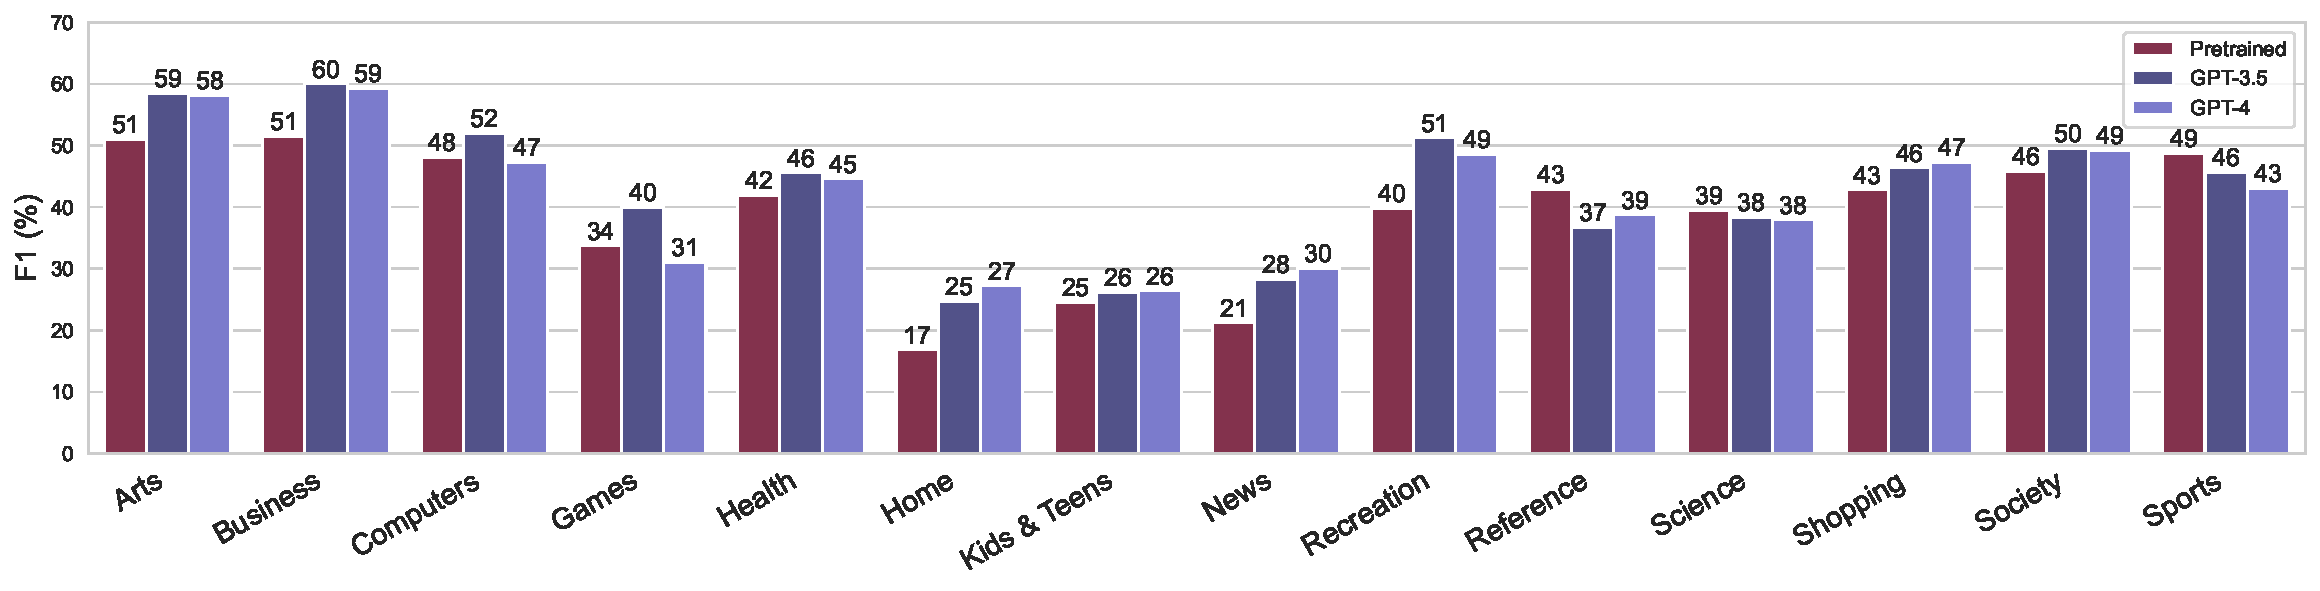
\includegraphics[width=\textwidth]{./figures/finetune-results.pdf}
    \caption{\textbf{Finetune Results.} Class-wise F1 score for the pre-trained model and the finetuned model on te original crowdsourced data.}
    \label{fig:finetune-results}
\end{figure*}


\subsection*{Phase 1: Identifying an Optimal LLM Labeler}

Table~\ref{tab:labeler-results} shows the results of re-labelling \texttt{crowdsourced} dataset. Our findings demonstrate that LLM labelers can provide \textit{consistent}, \textit{cost-effective}, and \textit{high-quality} annotations for the complex task of multilingual, multilabel website topic classification. 

% Consistency
Remarkably, not a single incorrect output was produced, underscoring the reliability the models in annotating websites.


% Cost
In terms of cost, the labeling of the \texttt{crowdsourced} corpus cost approximately \$130 per 1000 pages. Our approach, utilising GPT-3.5 and GPT-4 labelers, drastically reduces this cost to an average of \$0.54 and \$6.44, respectively, achieving a reduction by factors of 240x and 20x.

% Calculations
% Human annotator cost: 327 USD
% Pages annotated: 840 * 3 = 2520
% Cost per 1k page: 1000 * 327 / 2520 = 130$

% GPT-3.5 labler cost/1k pages:
% (0.36 + 0.48 + 0.42 + 0.63 + 0.57 + 0.80) / 6 = 0.54

% GPT-4 labler cost/1k pages:
% (4.68 + 5.75 + 5.26 + 7.25 + 6.68 + 8.99) / 6 = 6.44

% Cost reductions:
% GPT-3.5: 130 / 0.54 = 240x
% GPT-4: 130 / 6.44 = 20x

% Performance
Performance-wise, the best labeler, GPT-4 with \texttt{context3} and \texttt{1-shot}, achieves a macro F1 score of 46\% compared to the human annotations on the same dataset. Thus, the GPT labelers are better website classifiers than the baseline Homepage2Vec model, which achieves a macro F1 score of 39\% on the same dataset. This improvement gives us reason to believe that Homepage2Vec can learn from knowledge of the LLM labelers - the goal of the second phase of our study.


\begin{table}[!ht]
\centering
\caption{\textbf{Labeler Statistics}}
\label{tab:labeler-results}
\begin{tabular}{lllccc}
\toprule
 &  &  &  \textbf{LPP} & \textbf{Cost} & \textbf{M.-F1} \\
\textbf{Model} & \textbf{Context} & \textbf{Shot} & ($\mu\pm\sigma$) & (\$) & (\%) \\
\midrule
\multirow[c]{6}{*}{
    \rotatebox[origin=c]{90}{GPT-3.5}
    } & \multirow[c]{2}{*}{\texttt{context1}} & 0-shot & 0.39 ± 0.61 & \textbf{0.36} & 15.96 \\
 &  & 1-shot & 0.91 ± 0.95 & 0.48 & 23.26 \\
 & \multirow[c]{2}{*}{\texttt{context2}} & 0-shot & 1.39 ± 0.98 & 0.42 & 37.59 \\
 &  & 1-shot & 1.68 ± 1.15 & 0.63 & 38.69 \\
 & \multirow[c]{2}{*}{\texttt{context3}} & 0-shot & 1.57 ± 1.08 & 0.57 & 37.24 \\
 &  & 1-shot & 1.85 ± 1.24 & 0.80 & 37.70 \\
\midrule
\multirow[c]{6}{*}{
    \rotatebox[origin=c]{90}{GPT-4}
    } & \multirow[c]{2}{*}{\texttt{context1}} & 0-shot & 1.50 ± 0.93 & 4.68 & 35.55 \\
 &  & 1-shot & 1.83 ± 1.36 & 5.75 & 36.10 \\
 & \multirow[c]{2}{*}{\texttt{context2}} & 0-shot & 2.16 ± 1.03 & 5.26 & 45.39 \\
 &  & 1-shot & 2.49 ± 1.28 & 7.25 & 45.93 \\
 & \multirow[c]{2}{*}{\texttt{context3}} & 0-shot & 2.30 ± 1.11 & 6.68 & 44.10 \\
 &  & 1-shot & 2.80 ± 1.30 & 8.99 & \textbf{46.12} \\
\bottomrule
\end{tabular}
\end{table}


% GPT labeler parameter grid
\textbf{Labeler Parameter Grid.} Figure~\ref{fig:labelers-grid} visualises the effect of the labeler parameters on the annotation quality. As expected, we find that the quality of the labels increases with the amount of context provided and the complexity of the model used. Interestingly, the added features in \texttt{context3} (links and text) do not increase the annotation quality on average.


% Cost-quality trade-of
\textbf{Cost-Quality Trade-Off:} Our analysis reveals a positve trend between label quality and cost, attributable to the use of longer prompts or more sophisticated models. In the next phase, we aimed to select two labelers, one per model. In case of marginal improvements in label quality, we opted for the cheaper labeler. 
The best balance was achieved using \texttt{context2}; the GPT-3.5 labeler employed \texttt{1-shot}, whereas the GPT-4 used \texttt{0-shot}.

% Curlie-10k dataset
\textbf{Curlie-10k Dataset.} The average number of topics assigned to a page by the GPT 3.5 labeler is \textbf{1.6} and \textbf{2.03} for the GPT-4 labeler, which is both significantly than \textbf{1.07} for the original Curlie dataset. Figure~\ref{fig:curlie-10k-dist} shows the distribution of the labels in the re-labelled dataset compared to the original. We can see that, as hoped, more topics are assigned to each page. Interesting differences in the GPT-3.5 and GPT-4 labelers visible: the GPT-4 labeler tends to assign more websites to the topics that are less frequent in the original dataset, such as \textit{References}, \textit{Kids \& Teens} and \textit{Games}, leading to a more balanced distribution of topics. Surprisingly, the category \textit{Recreation} is assigned to a disproportionally high number of websites by the GPT-4 labeler.

\begin{figure}[!ht]
    \centering
    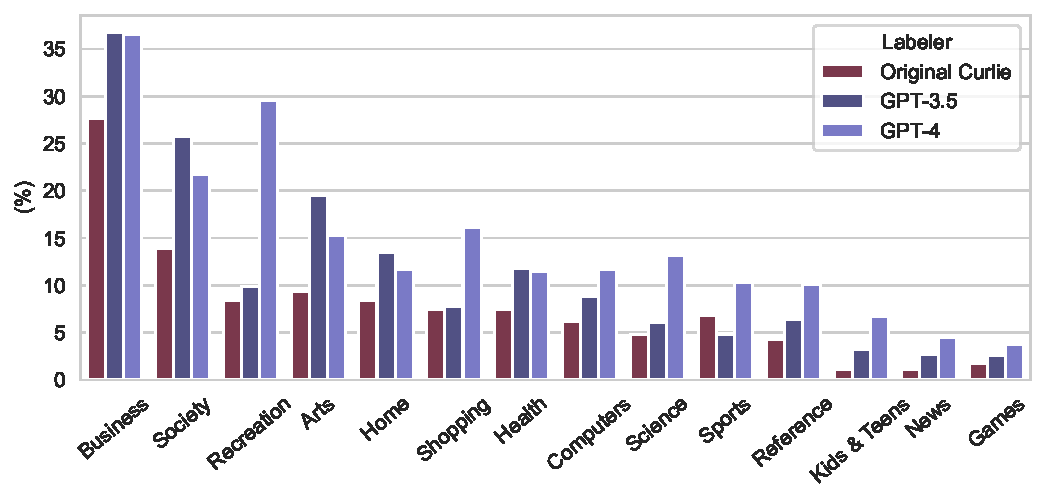
\includegraphics[width=.8\columnwidth]{figures/curlie-10k-dist.pdf}
    \caption{\textbf{Curlie-10k Label Distribution.} Topic distribution of \texttt{curlie-gpt3.5-10k}, \texttt{curlie-gpt4-10k}, as well as \texttt{curlie} for reference.}
    \label{fig:curlie-10k-dist}
\end{figure}

\subsection*{Phase 2: Transferring Knowledge via Finetuning}

Table~\ref{tab:finetune-results} shows the results of the finetuning experiments. 
We observe that the model increases the recall significantly from 39.4\% to 47.6\% and /49\% when finetuned on GPT-3.5 and GPT-4 labels, respectively.
However, this comes at cost of a minor decreases in precision. Overall, the macro F1 score from increases from 39.2\% to 42.6\% and 42.8\% - an improvement of 3.4 and 3.6 percentage points, respectively.
This improvement shows that we were able to transfer the superior labeling capabilities of the LLM to Homepage2Vec, by finetuning on LLM-generated labels. Figure~\ref{fig:finetune-results} shows that the increase in macro F1 score is achieved by consistently acrosss the classes, with 12 out of the 14 classes improving.

% 0.391610 = 39.2% (Pre-trained Homepage2Vec)
% 0.426289 = 42.6% (GPT-3.5) (+3.4 percentage points)
% 0.428    = 42.8% (GPT-4) (+3.6 percentage points)

\begin{table}[!ht]
\centering
\caption{\textbf{Finetuning Results.} The table shows the precision, recall, macro F1 and and labels per page when evaluated on \texttt{crowdsourced}. We show results for the pre-trained baseline, as well as both finetuned variants.}
\label{tab:finetune-results}
\begin{tabular}{lrrrr}
\toprule
 & \textbf{Pr.} & \textbf{Re.} & \textbf{M.-F1} & \textbf{LPP} \\
 & (\%) & (\%) & (\%) & ($\mu$) \\
\midrule
Pretrained & \textbf{40.97} & 39.44 & 39.16 & 1.84 \\
GPT-3.5 & 40.19 & 47.55 & 42.63 & 1.93 \\
GPT-4 & 39.92 & \textbf{49.07} & \textbf{42.87} & \textbf{3.07} \\
\bottomrule
\end{tabular}
\end{table}


